\subsection{Main comparison: four published devices and the memistor}\label{sec:main}
Table~\ref{tab:main} and Fig.~\ref{fig:main} give the gap to the exact-update baseline over five seeds.

\paragraph{Plain SGD fails.} On every published electrochemical device, plain SGD lies wholly above the line on all three tasks
(\REThreeMnistSgdNfail, \REThreeCifarSgdNfail{} and \REThreeLmSgdNfail{} of four devices FAIL on MNIST, CIFAR and the LM). This
holds even though the Li-ECRAM, protonic and metal-oxide specifications have about a thousand or more levels. Their asymmetric,
saturating steps pull the weights toward their symmetry points, as predicted by~\cite{gokmen2020,wu2025}.

\paragraph{The Tiki-Taka family recovers most of the gap.}
\begin{itemize}
\item \textbf{Best cell per task} among the published devices:
      \begin{itemize}
      \item MNIST: \REThreeMnistBestDev{} with \REThreeMnistBestAlgo, \REThreeMnistBestGap\,pp
            [\REThreeMnistBestLo, \REThreeMnistBestHi], \REThreeMnistBestLabel;
      \item CIFAR: \REThreeCifarBestDev{} with \REThreeCifarBestAlgo, \REThreeCifarBestGap\,pp
            [\REThreeCifarBestLo, \REThreeCifarBestHi], \REThreeCifarBestLabel;
      \item LM: \REThreeLmBestDev{} with \REThreeLmBestAlgo, \REThreeLmBestGap\%
            [\REThreeLmBestLo, \REThreeLmBestHi], \REThreeLmBestLabel.
      \end{itemize}
\item \textbf{Strictest reading} (whole interval below the line on every task):
      \begin{itemize}
      \item Mixing algorithms across tasks, \REThreeNpassall{} devices pass all three tasks: \REThreePassallList.
      \item With one algorithm on all three tasks, \REThreeSameNpass{} pairings pass everywhere.
      \end{itemize}
\item \textbf{No cell fails.} \REThreeSameNnofail{} device--algorithm pairings have no FAIL on any task: \REThreeSameNofailList.
      Their remaining cells are UNRESOLVED: the interval contains the line.
\end{itemize}

The limiting factor is statistical as well as physical. On the CIFAR subset the FP baseline itself varies by
\REThreeCifarFpSd\,pp (standard deviation over seeds), so five seeds give intervals about $\pm2$\,pp wide.

\paragraph{The devices separate clearly.}
\begin{itemize}
\item \textbf{Li-ECRAM and protonic} are within or near the lines.
\item \textbf{Metal-oxide ECRAM} is good on MNIST but fails on the LM. Its fitted write noise is twice its (very small) step.
\item \textbf{W/YSZ/WO$_x$} fails on CIFAR and the LM with every algorithm. Its 256 states and strong nonlinearity are not
      enough for these tasks, although they suffice for its published $10\times10$ demonstration.
\item \textbf{Widrow's memistor, as he described it} (thousands of levels, near-linear), does as well as the modern devices on
      MNIST, where even plain SGD passes on it because his description implies an almost symmetric device. On the LM it sits between the good and the poor modern devices.
\end{itemize}
The memistor's ideal was right; what the 1960 device lacked was density, speed and energy, not accuracy
(Section~\ref{sec:energy}).

\paragraph{Among the tolerant algorithms.}
\begin{itemize}
\item c-TTv2 gives the best LM results on Li-ECRAM and protonic devices.
\item AGAD is the most uniform on MNIST, but it is not uniformly better. On the noisiest device (metal-oxide) AGAD is the best
      tolerant algorithm on the LM, while on the coarse 20-state device of Section~\ref{sec:validation} it pays an accuracy
      cost.
\item Plain TTv2, our pre-registered choice for the specification sheet because it scored best on validation, is not the best
      on the LM for any device except, marginally, W/YSZ/WO$_x$, where every algorithm fails.
\end{itemize}

\paragraph{Against Adam.} The pre-registered baseline is SGD with an exact update. For context, the FP-SGD language model is
\REThreeLmFpvsadam\% worse in bits per byte than the same network trained by Adam in digital. The best analog cells are about as
far from Adam as FP-SGD is. Analog training here inherits SGD's optimiser gap; closing that gap needs analog-friendly adaptive
methods, which are beyond this study.

% generated by analyze.py (do not edit)
\begin{table*}[t]\centering\footnotesize
\caption{Main result (E3): gap to the exact-update baseline, mean and 95\% t-interval over 5 seeds, paired by seed. MNIST and CIFAR in percentage points of test accuracy; LM in \% of bits per byte. P = the whole interval is below the line (2 pp; 5\%), F = wholly above, U = the interval contains the line. Every arm uses the FP validation learning rate.}\label{tab:main}
\fitbox{\begin{tabular}{llccc}\toprule
Device & Algorithm & MNIST gap (pp) & CIFAR-10 subset gap (pp) & char-LM gap (\%)\\\midrule
\multicolumn{2}{l}{FP baseline (acc.\ \%; bpb)} & 97.85 [97.79, 97.92] & 60.39 [58.64, 62.14] & 2.912 [2.822, 3.001]\\\midrule
Li-ECRAM (Tang 2018) & SGD & 4.85 [4.73, 4.98] F & 20.81 [18.06, 23.57] F & 45.58 [31.52, 59.64] F\\
 & TTv2 & 1.32 [0.49, 2.14] U & 2.95 [0.94, 4.96] U & 3.52 [0.86, 6.18] U\\
 & c-TTv2 & 1.79 [0.94, 2.65] U & 0.10 [-1.27, 1.47] P & -1.29 [-4.46, 1.87] P\\
 & AGAD & 0.86 [0.67, 1.06] P & 1.06 [-1.05, 3.17] U & 3.60 [-0.09, 7.30] U\\
\midrule
MO-ECRAM (Kim 2019) & SGD & 6.96 [6.60, 7.31] F & 25.29 [22.15, 28.44] F & 50.84 [36.24, 65.45] F\\
 & TTv2 & 1.80 [1.68, 1.91] P & 5.45 [2.15, 8.75] F & 16.51 [13.17, 19.84] F\\
 & c-TTv2 & 1.90 [1.81, 1.99] P & 1.94 [-0.15, 4.03] U & 15.68 [7.21, 24.14] F\\
 & AGAD & 0.49 [0.33, 0.66] P & 1.39 [-0.31, 3.09] U & 8.88 [6.10, 11.65] F\\
\midrule
Protonic (Onen 2022) & SGD & 3.07 [2.85, 3.29] F & 15.77 [10.75, 20.79] F & 40.82 [34.31, 47.33] F\\
 & TTv2 & 1.04 [0.40, 1.69] P & 2.13 [0.49, 3.77] U & 3.64 [0.98, 6.30] U\\
 & c-TTv2 & 0.74 [0.44, 1.05] P & 0.08 [-2.57, 2.73] U & -0.84 [-4.30, 2.62] P\\
 & AGAD & 1.17 [0.73, 1.62] P & 0.56 [-0.85, 1.98] P & 3.82 [0.32, 7.33] U\\
\midrule
W/YSZ/WO$_x$ (Chen 2023) & SGD & 8.25 [7.47, 9.02] F & 36.82 [33.17, 40.47] F & 50.67 [47.53, 53.81] F\\
 & TTv2 & 1.48 [1.37, 1.60] P & 10.59 [8.94, 12.24] F & 21.17 [17.11, 25.24] F\\
 & c-TTv2 & 1.75 [1.33, 2.17] U & 9.87 [7.90, 11.84] F & 21.23 [17.81, 24.66] F\\
 & AGAD & 1.08 [0.79, 1.37] P & 17.55 [15.52, 19.58] F & 26.59 [20.81, 32.38] F\\
\midrule
Memistor (Widrow 1960, as claimed) & SGD & 1.29 [1.12, 1.46] P & 9.86 [2.80, 16.92] F & 30.94 [25.31, 36.57] F\\
 & TTv2 & 0.73 [0.28, 1.17] P & 2.86 [-0.64, 6.35] U & 8.99 [5.43, 12.54] F\\
 & c-TTv2 & 0.49 [0.21, 0.77] P & 1.32 [0.08, 2.55] U & 6.59 [1.96, 11.23] U\\
 & AGAD & 1.29 [0.64, 1.94] P & 2.06 [0.68, 3.44] U & 7.76 [3.53, 11.99] U\\
\bottomrule\end{tabular}}\end{table*}

\begin{figure}[t]\centering
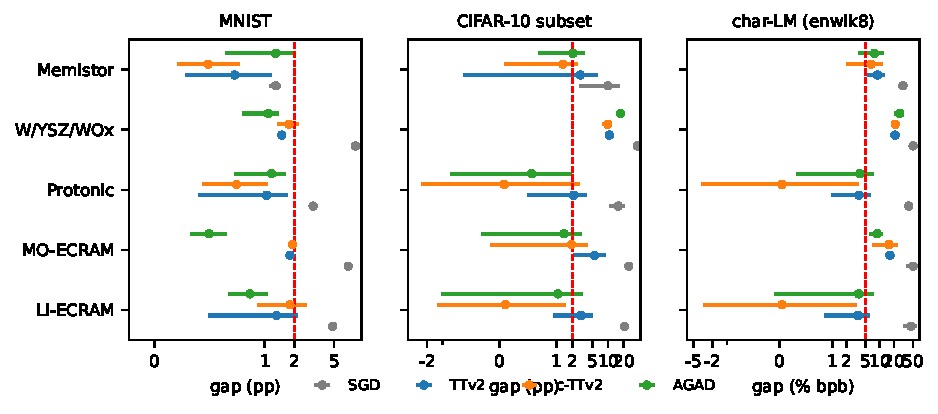
\includegraphics[width=\linewidth]{figs/fig_main}
\caption{Gap to the exact-update baseline (mean and 95\% interval over 5 seeds; symmetric-log axis); the dashed line is the
pre-registered gap line.}\label{fig:main}
\end{figure}
